\section{Sección Uno}
\subsection{Apartado Uno}

Texto del apartado uno, y referenciando a
	Knuth\cite{knuth97,knuth:1984,texbook}, y
	otros\cite{latex:companion,latex2e,lesk:1977} o el kernel de
	linux\cite{Kernel:GitHub}

\begin{itemize}
   \item Item 1
   \item Item 2
   \item Item 3
   \item Item 4
\end{itemize}


\section{Sección Dos}


\begin{itemize}
   \item Item 1
   \item Item 2
   \item Item 3
\end{itemize}


\section{Sección Tres}


Bla, bla, bla.


\section{Sección Cuatro}


Bla, bla, bla.


\newpage

\begin{figure}[htb]
   \centering
   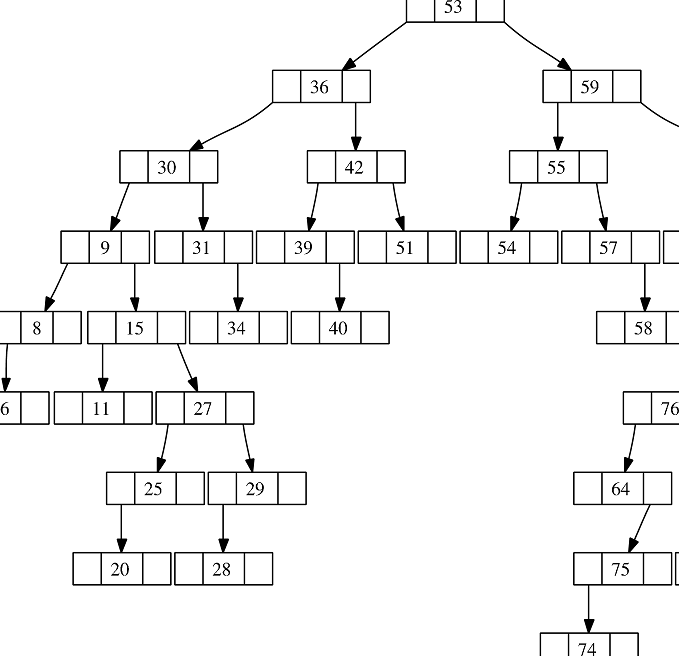
\includegraphics[width=0.7\textwidth]{images/figura_1}
   \caption{Ejemplo de figura}
   \label{fig:ejemplo}
\end{figure}


\begin{lstlisting}[language=json,firstnumber=1,caption={Un listado},label={code:ejemplo}]
{"menu": {
  "id": "file",
  "value": "File",
  "popup": {
    "menuitem": [
      {"value": "New", "onclick": "CreateNewDoc()"},
      {"value": "Open", "onclick": "OpenDoc()"},
      {"value": "Close", "onclick": "CloseDoc()"}
    ]
  }
}}
0123456789
\end{lstlisting}
